\documentclass[1p]{elsarticle_modified}
%\bibliographystyle{elsarticle-num}

%\usepackage[colorlinks]{hyperref}
%\usepackage{abbrmath_seonhwa} %\Abb, \Ascr, \Acal ,\Abf, \Afrak
\usepackage{amsfonts}
\usepackage{amssymb}
\usepackage{amsmath}
\usepackage{amsthm}
\usepackage{scalefnt}
\usepackage{amsbsy}
\usepackage{kotex}
\usepackage{caption}
\usepackage{subfig}
\usepackage{color}
\usepackage{graphicx}
\usepackage{xcolor} %% white, black, red, green, blue, cyan, magenta, yellow
\usepackage{float}
\usepackage{setspace}
\usepackage{hyperref}

\usepackage{tikz}
\usetikzlibrary{arrows}

\usepackage{multirow}
\usepackage{array} % fixed length table
\usepackage{hhline}

%%%%%%%%%%%%%%%%%%%%%
\makeatletter
\renewcommand*\env@matrix[1][\arraystretch]{%
	\edef\arraystretch{#1}%
	\hskip -\arraycolsep
	\let\@ifnextchar\new@ifnextchar
	\array{*\c@MaxMatrixCols c}}
\makeatother %https://tex.stackexchange.com/questions/14071/how-can-i-increase-the-line-spacing-in-a-matrix
%%%%%%%%%%%%%%%

\usepackage[normalem]{ulem}

\newcommand{\msout}[1]{\ifmmode\text{\sout{\ensuremath{#1}}}\else\sout{#1}\fi}
%SOURCE: \msout is \stkout macro in https://tex.stackexchange.com/questions/20609/strikeout-in-math-mode

\newcommand{\cancel}[1]{
	\ifmmode
	{\color{red}\msout{#1}}
	\else
	{\color{red}\sout{#1}}
	\fi
}

\newcommand{\add}[1]{
	{\color{blue}\uwave{#1}}
}

\newcommand{\replace}[2]{
	\ifmmode
	{\color{red}\msout{#1}}{\color{blue}\uwave{#2}}
	\else
	{\color{red}\sout{#1}}{\color{blue}\uwave{#2}}
	\fi
}

\newcommand{\Sol}{\mathcal{S}} %segment
\newcommand{\D}{D} %diagram
\newcommand{\A}{\mathcal{A}} %arc


%%%%%%%%%%%%%%%%%%%%%%%%%%%%%5 test

\def\sl{\operatorname{\textup{SL}}(2,\Cbb)}
\def\psl{\operatorname{\textup{PSL}}(2,\Cbb)}
\def\quan{\mkern 1mu \triangleright \mkern 1mu}

\theoremstyle{definition}
\newtheorem{thm}{Theorem}[section]
\newtheorem{prop}[thm]{Proposition}
\newtheorem{lem}[thm]{Lemma}
\newtheorem{ques}[thm]{Question}
\newtheorem{cor}[thm]{Corollary}
\newtheorem{defn}[thm]{Definition}
\newtheorem{exam}[thm]{Example}
\newtheorem{rmk}[thm]{Remark}
\newtheorem{alg}[thm]{Algorithm}

\newcommand{\I}{\sqrt{-1}}
\begin{document}

%\begin{frontmatter}
%
%\title{Boundary parabolic representations of knots up to 8 crossings}
%
%%% Group authors per affiliation:
%\author{Yunhi Cho} 
%\address{Department of Mathematics, University of Seoul, Seoul, Korea}
%\ead{yhcho@uos.ac.kr}
%
%
%\author{Seonhwa Kim} %\fnref{s_kim}}
%\address{Center for Geometry and Physics, Institute for Basic Science, Pohang, 37673, Korea}
%\ead{ryeona17@ibs.re.kr}
%
%\author{Hyuk Kim}
%\address{Department of Mathematical Sciences, Seoul National University, Seoul 08826, Korea}
%\ead{hyukkim@snu.ac.kr}
%
%\author{Seokbeom Yoon}
%\address{Department of Mathematical Sciences, Seoul National University, Seoul, 08826,  Korea}
%\ead{sbyoon15@snu.ac.kr}
%
%\begin{abstract}
%We find all boundary parabolic representation of knots up to 8 crossings.
%
%\end{abstract}
%\begin{keyword}
%    \MSC[2010] 57M25 
%\end{keyword}
%
%\end{frontmatter}

%\linenumbers
%\tableofcontents
%
\newcommand\colored[1]{\textcolor{white}{\rule[-0.35ex]{0.8em}{1.4ex}}\kern-0.8em\color{red} #1}%
%\newcommand\colored[1]{\textcolor{white}{ #1}\kern-2.17ex	\textcolor{white}{ #1}\kern-1.81ex	\textcolor{white}{ #1}\kern-2.15ex\color{red}#1	}

{\Large $\underline{12a_{1094}~(K12a_{1094})}$}

\setlength{\tabcolsep}{10pt}
\renewcommand{\arraystretch}{1.6}
\vspace{1cm}\begin{tabular}{m{100pt}>{\centering\arraybackslash}m{274pt}}
\multirow{5}{120pt}{
	\centering
	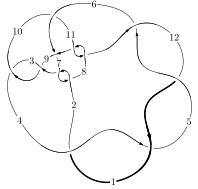
\includegraphics[width=112pt]{../../../GIT/diagram.site/Diagrams/png/1895_12a_1094.png}\\
\ \ \ A knot diagram\footnotemark}&
\allowdisplaybreaks
\textbf{Linearized knot diagam} \\
\cline{2-2}
 &
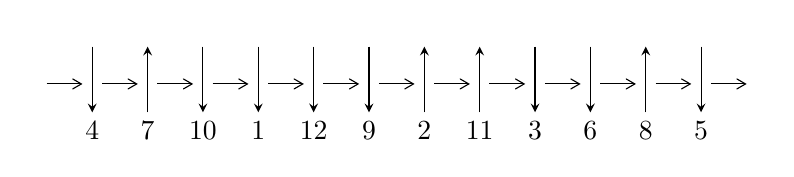
\begin{tikzpicture}[x=20pt, y=17pt]
	% nodes
	\node (C0) at (0, 0) {};
	\node (C1) at (1, 0) {};
	\node (C1U) at (1, +1) {};
	\node (C1D) at (1, -1) {4};

	\node (C2) at (2, 0) {};
	\node (C2U) at (2, +1) {};
	\node (C2D) at (2, -1) {7};

	\node (C3) at (3, 0) {};
	\node (C3U) at (3, +1) {};
	\node (C3D) at (3, -1) {10};

	\node (C4) at (4, 0) {};
	\node (C4U) at (4, +1) {};
	\node (C4D) at (4, -1) {1};

	\node (C5) at (5, 0) {};
	\node (C5U) at (5, +1) {};
	\node (C5D) at (5, -1) {12};

	\node (C6) at (6, 0) {};
	\node (C6U) at (6, +1) {};
	\node (C6D) at (6, -1) {9};

	\node (C7) at (7, 0) {};
	\node (C7U) at (7, +1) {};
	\node (C7D) at (7, -1) {2};

	\node (C8) at (8, 0) {};
	\node (C8U) at (8, +1) {};
	\node (C8D) at (8, -1) {11};

	\node (C9) at (9, 0) {};
	\node (C9U) at (9, +1) {};
	\node (C9D) at (9, -1) {3};

	\node (C10) at (10, 0) {};
	\node (C10U) at (10, +1) {};
	\node (C10D) at (10, -1) {6};

	\node (C11) at (11, 0) {};
	\node (C11U) at (11, +1) {};
	\node (C11D) at (11, -1) {8};

	\node (C12) at (12, 0) {};
	\node (C12U) at (12, +1) {};
	\node (C12D) at (12, -1) {5};
	\node (C13) at (13, 0) {};

	% arrows
	\draw[->,>={angle 60}]
	(C0) edge (C1) (C1) edge (C2) (C2) edge (C3) (C3) edge (C4) (C4) edge (C5) (C5) edge (C6) (C6) edge (C7) (C7) edge (C8) (C8) edge (C9) (C9) edge (C10) (C10) edge (C11) (C11) edge (C12) (C12) edge (C13) ;	\draw[->,>=stealth]
	(C1U) edge (C1D) (C2D) edge (C2U) (C3U) edge (C3D) (C4U) edge (C4D) (C5U) edge (C5D) (C6U) edge (C6D) (C7D) edge (C7U) (C8D) edge (C8U) (C9U) edge (C9D) (C10U) edge (C10D) (C11D) edge (C11U) (C12U) edge (C12D) ;
	\end{tikzpicture} \\
\hhline{~~} \\& 
\textbf{Solving Sequence} \\ \cline{2-2} 
 &
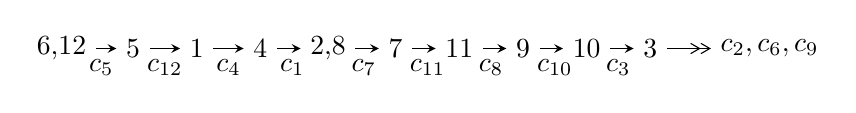
\begin{tikzpicture}[x=23pt, y=7pt]
	% node
	\node (A0) at (-1/8, 0) {6,12};
	\node (A1) at (1, 0) {5};
	\node (A2) at (2, 0) {1};
	\node (A3) at (3, 0) {4};
	\node (A4) at (65/16, 0) {2,8};
	\node (A5) at (41/8, 0) {7};
	\node (A6) at (49/8, 0) {11};
	\node (A7) at (57/8, 0) {9};
	\node (A8) at (65/8, 0) {10};
	\node (A9) at (73/8, 0) {3};
	\node (C1) at (1/2, -1) {$c_{5}$};
	\node (C2) at (3/2, -1) {$c_{12}$};
	\node (C3) at (5/2, -1) {$c_{4}$};
	\node (C4) at (7/2, -1) {$c_{1}$};
	\node (C5) at (37/8, -1) {$c_{7}$};
	\node (C6) at (45/8, -1) {$c_{11}$};
	\node (C7) at (53/8, -1) {$c_{8}$};
	\node (C8) at (61/8, -1) {$c_{10}$};
	\node (C9) at (69/8, -1) {$c_{3}$};
	\node (A10) at (11, 0) {$c_{2},c_{6},c_{9}$};

	% edge
	\draw[->,>=stealth]	
	(A0) edge (A1) (A1) edge (A2) (A2) edge (A3) (A3) edge (A4) (A4) edge (A5) (A5) edge (A6) (A6) edge (A7) (A7) edge (A8) (A8) edge (A9) ;
	\draw[->>,>={angle 60}]	
	(A9) edge (A10);
\end{tikzpicture} \\ 

\end{tabular} \\

\footnotetext{
The image of knot diagram is generated by the software ``\textbf{Draw programme}" developed by Andrew Bartholomew(\url{http://www.layer8.co.uk/maths/draw/index.htm\#Running-draw}), where we modified some parts for our purpose(\url{https://github.com/CATsTAILs/LinksPainter}).
}\phantom \\ \newline 
\centering \textbf{Ideals for irreducible components\footnotemark of $X_{\text{par}}$} 
 
\begin{align*}
I^u_{1}&=\langle 
6.83030\times10^{106} u^{89}+1.55405\times10^{107} u^{88}+\cdots+6.21904\times10^{106} b+7.24350\times10^{106},\\
\phantom{I^u_{1}}&\phantom{= \langle  }1.29538\times10^{107} u^{89}+3.57847\times10^{107} u^{88}+\cdots+6.21904\times10^{106} a+6.18948\times10^{106},\;u^{90}+3 u^{89}+\cdots+12 u+1\rangle \\
I^u_{2}&=\langle 
u^{22}+2 u^{21}+\cdots+b-1,\;u^{23}+2 u^{22}+\cdots+a-7,\;u^{24}+2 u^{23}+\cdots+17 u^2+1\rangle \\
I^u_{3}&=\langle 
u^2+b,\;a-1,\;u^7+3 u^5+2 u^3+u-1\rangle \\
\\
\end{align*}
\raggedright * 3 irreducible components of $\dim_{\mathbb{C}}=0$, with total 121 representations.\\
\footnotetext{All coefficients of polynomials are rational numbers. But the coefficients are sometimes approximated in decimal forms when there is not enough margin.}
\newpage
\renewcommand{\arraystretch}{1}
\centering \section*{I. $I^u_{1}= \langle 6.83\times10^{106} u^{89}+1.55\times10^{107} u^{88}+\cdots+6.22\times10^{106} b+7.24\times10^{106},\;1.30\times10^{107} u^{89}+3.58\times10^{107} u^{88}+\cdots+6.22\times10^{106} a+6.19\times10^{106},\;u^{90}+3 u^{89}+\cdots+12 u+1 \rangle$}
\flushleft \textbf{(i) Arc colorings}\\
\begin{tabular}{m{7pt} m{180pt} m{7pt} m{180pt} }
\flushright $a_{6}=$&$\begin{pmatrix}1\\0\end{pmatrix}$ \\
\flushright $a_{12}=$&$\begin{pmatrix}0\\u\end{pmatrix}$ \\
\flushright $a_{5}=$&$\begin{pmatrix}1\\- u^2\end{pmatrix}$ \\
\flushright $a_{1}=$&$\begin{pmatrix}- u\\u^3+u\end{pmatrix}$ \\
\flushright $a_{4}=$&$\begin{pmatrix}u^2+1\\- u^4-2 u^2\end{pmatrix}$ \\
\flushright $a_{2}=$&$\begin{pmatrix}- u^3-2 u\\u^5+3 u^3+u\end{pmatrix}$ \\
\flushright $a_{8}=$&$\begin{pmatrix}-2.08292 u^{89}-5.75405 u^{88}+\cdots-103.537 u-0.995248\\-1.09829 u^{89}-2.49885 u^{88}+\cdots-36.1802 u-1.16473\end{pmatrix}$ \\
\flushright $a_{7}=$&$\begin{pmatrix}-2.30239 u^{89}-5.89176 u^{88}+\cdots-92.0794 u+0.607952\\-0.686489 u^{89}-1.62055 u^{88}+\cdots-35.8591 u-1.44130\end{pmatrix}$ \\
\flushright $a_{11}=$&$\begin{pmatrix}-0.0309762 u^{89}-0.977314 u^{88}+\cdots-81.9158 u-10.9345\\-1.14038 u^{89}-3.23467 u^{88}+\cdots-35.2548 u-4.73665\end{pmatrix}$ \\
\flushright $a_{9}=$&$\begin{pmatrix}3.07250 u^{89}+8.58048 u^{88}+\cdots+42.3487 u+8.12578\\0.0736579 u^{89}-0.256335 u^{88}+\cdots-40.1867 u-2.49488\end{pmatrix}$ \\
\flushright $a_{10}=$&$\begin{pmatrix}-1.17135 u^{89}-4.21198 u^{88}+\cdots-117.171 u-15.6711\\-1.14038 u^{89}-3.23467 u^{88}+\cdots-35.2548 u-4.73665\end{pmatrix}$ \\
\flushright $a_{3}=$&$\begin{pmatrix}-3.38625 u^{89}-10.3318 u^{88}+\cdots-155.927 u-20.4178\\-1.23019 u^{89}-3.17312 u^{88}+\cdots-10.9793 u-2.96508\end{pmatrix}$\\&\end{tabular}
\flushleft \textbf{(ii) Obstruction class $= -1$}\\~\\
\flushleft \textbf{(iii) Cusp Shapes $= 0.162569 u^{89}-3.73818 u^{88}+\cdots-145.744 u-28.3707$}\\~\\
\newpage\renewcommand{\arraystretch}{1}
\flushleft \textbf{(iv) u-Polynomials at the component}\newline \\
\begin{tabular}{m{50pt}|m{274pt}}
Crossings & \hspace{64pt}u-Polynomials at each crossing \\
\hline $$\begin{aligned}c_{1},c_{4},c_{5}\\c_{12}\end{aligned}$$&$\begin{aligned}
&u^{90}-3 u^{89}+\cdots-12 u+1
\end{aligned}$\\
\hline $$\begin{aligned}c_{2},c_{7}\end{aligned}$$&$\begin{aligned}
&u^{90}+u^{89}+\cdots-1472 u+37417
\end{aligned}$\\
\hline $$\begin{aligned}c_{3},c_{9}\end{aligned}$$&$\begin{aligned}
&u^{90}-6 u^{89}+\cdots-13860 u+2776
\end{aligned}$\\
\hline $$\begin{aligned}c_{6}\end{aligned}$$&$\begin{aligned}
&u^{90}-5 u^{89}+\cdots-305292 u+114001
\end{aligned}$\\
\hline $$\begin{aligned}c_{8},c_{11}\end{aligned}$$&$\begin{aligned}
&u^{90}+5 u^{89}+\cdots+7842 u+839
\end{aligned}$\\
\hline $$\begin{aligned}c_{10}\end{aligned}$$&$\begin{aligned}
&u^{90}+u^{89}+\cdots+13461 u+2479
\end{aligned}$\\
\hline
\end{tabular}\\~\\
\newpage\renewcommand{\arraystretch}{1}
\flushleft \textbf{(v) Riley Polynomials at the component}\newline \\
\begin{tabular}{m{50pt}|m{274pt}}
Crossings & \hspace{64pt}Riley Polynomials at each crossing \\
\hline $$\begin{aligned}c_{1},c_{4},c_{5}\\c_{12}\end{aligned}$$&$\begin{aligned}
&y^{90}+109 y^{89}+\cdots+174 y+1
\end{aligned}$\\
\hline $$\begin{aligned}c_{2},c_{7}\end{aligned}$$&$\begin{aligned}
&y^{90}+65 y^{89}+\cdots+22616709052 y+1400031889
\end{aligned}$\\
\hline $$\begin{aligned}c_{3},c_{9}\end{aligned}$$&$\begin{aligned}
&y^{90}-58 y^{89}+\cdots-11659600 y+7706176
\end{aligned}$\\
\hline $$\begin{aligned}c_{6}\end{aligned}$$&$\begin{aligned}
&y^{90}-45 y^{89}+\cdots-374166877836 y+12996228001
\end{aligned}$\\
\hline $$\begin{aligned}c_{8},c_{11}\end{aligned}$$&$\begin{aligned}
&y^{90}+53 y^{89}+\cdots+29423788 y+703921
\end{aligned}$\\
\hline $$\begin{aligned}c_{10}\end{aligned}$$&$\begin{aligned}
&y^{90}-19 y^{89}+\cdots-310592405 y+6145441
\end{aligned}$\\
\hline
\end{tabular}\\~\\
\newpage\flushleft \textbf{(vi) Complex Volumes and Cusp Shapes}
$$\begin{array}{c|c|c}  
\text{Solutions to }I^u_{1}& \I (\text{vol} + \sqrt{-1}CS) & \text{Cusp shape}\\
 \hline 
\begin{aligned}
u &= -0.673798 + 0.745251 I \\
a &= \phantom{-}0.59357 - 1.29182 I \\
b &= \phantom{-}0.71141 + 1.77487 I\end{aligned}
 & -7.3826 + 13.2885 I & \phantom{-0.000000 } 0 \\ \hline\begin{aligned}
u &= -0.673798 - 0.745251 I \\
a &= \phantom{-}0.59357 + 1.29182 I \\
b &= \phantom{-}0.71141 - 1.77487 I\end{aligned}
 & -7.3826 - 13.2885 I & \phantom{-0.000000 } 0 \\ \hline\begin{aligned}
u &= -0.318813 + 0.972274 I \\
a &= \phantom{-}0.354309 - 0.417115 I \\
b &= \phantom{-}1.29131 + 0.58699 I\end{aligned}
 & -1.92726 - 1.07654 I & \phantom{-0.000000 } 0 \\ \hline\begin{aligned}
u &= -0.318813 - 0.972274 I \\
a &= \phantom{-}0.354309 + 0.417115 I \\
b &= \phantom{-}1.29131 - 0.58699 I\end{aligned}
 & -1.92726 + 1.07654 I & \phantom{-0.000000 } 0 \\ \hline\begin{aligned}
u &= \phantom{-}0.554780 + 0.764528 I \\
a &= \phantom{-}0.78623 + 1.29463 I \\
b &= \phantom{-}0.56005 - 1.47151 I\end{aligned}
 & -3.13661 - 7.27639 I & \phantom{-0.000000 } 0 \\ \hline\begin{aligned}
u &= \phantom{-}0.554780 - 0.764528 I \\
a &= \phantom{-}0.78623 - 1.29463 I \\
b &= \phantom{-}0.56005 + 1.47151 I\end{aligned}
 & -3.13661 + 7.27639 I & \phantom{-0.000000 } 0 \\ \hline\begin{aligned}
u &= \phantom{-}0.623759 + 0.627084 I \\
a &= -0.507263 - 0.842395 I \\
b &= -0.275207 + 1.385920 I\end{aligned}
 & -0.99512 - 2.46332 I & \phantom{-0.000000 } 0 \\ \hline\begin{aligned}
u &= \phantom{-}0.623759 - 0.627084 I \\
a &= -0.507263 + 0.842395 I \\
b &= -0.275207 - 1.385920 I\end{aligned}
 & -0.99512 + 2.46332 I & \phantom{-0.000000 } 0 \\ \hline\begin{aligned}
u &= -0.842119 + 0.262679 I \\
a &= -0.89625 + 1.19447 I \\
b &= \phantom{-}0.10031 - 1.55471 I\end{aligned}
 & -8.85310 - 8.28939 I & \phantom{-0.000000 } 0 \\ \hline\begin{aligned}
u &= -0.842119 - 0.262679 I \\
a &= -0.89625 - 1.19447 I \\
b &= \phantom{-}0.10031 + 1.55471 I\end{aligned}
 & -8.85310 + 8.28939 I & \phantom{-0.000000 } 0\\
 \hline 
 \end{array}$$\newpage$$\begin{array}{c|c|c}  
\text{Solutions to }I^u_{1}& \I (\text{vol} + \sqrt{-1}CS) & \text{Cusp shape}\\
 \hline 
\begin{aligned}
u &= \phantom{-}0.333793 + 0.814040 I \\
a &= \phantom{-}0.333808 - 0.618859 I \\
b &= -0.397603 + 0.240312 I\end{aligned}
 & \phantom{-}0.82127 - 2.96271 I & \phantom{-0.000000 } 0 \\ \hline\begin{aligned}
u &= \phantom{-}0.333793 - 0.814040 I \\
a &= \phantom{-}0.333808 + 0.618859 I \\
b &= -0.397603 - 0.240312 I\end{aligned}
 & \phantom{-}0.82127 + 2.96271 I & \phantom{-0.000000 } 0 \\ \hline\begin{aligned}
u &= -0.728004 + 0.474895 I \\
a &= -0.012276 + 1.177780 I \\
b &= -0.64564 - 1.47165 I\end{aligned}
 & -2.24160 + 4.56943 I & \phantom{-0.000000 } 0 \\ \hline\begin{aligned}
u &= -0.728004 - 0.474895 I \\
a &= -0.012276 - 1.177780 I \\
b &= -0.64564 + 1.47165 I\end{aligned}
 & -2.24160 - 4.56943 I & \phantom{-0.000000 } 0 \\ \hline\begin{aligned}
u &= \phantom{-}0.482332 + 1.026280 I \\
a &= -0.881390 - 0.301898 I \\
b &= -0.096950 + 1.030020 I\end{aligned}
 & -1.64550 - 1.00721 I & \phantom{-0.000000 } 0 \\ \hline\begin{aligned}
u &= \phantom{-}0.482332 - 1.026280 I \\
a &= -0.881390 + 0.301898 I \\
b &= -0.096950 - 1.030020 I\end{aligned}
 & -1.64550 + 1.00721 I & \phantom{-0.000000 } 0 \\ \hline\begin{aligned}
u &= \phantom{-}0.460781 + 0.723596 I \\
a &= -0.95388 - 1.13852 I \\
b &= -0.92691 + 1.88015 I\end{aligned}
 & -2.60445 - 6.80426 I & \phantom{-0.000000 } 0 \\ \hline\begin{aligned}
u &= \phantom{-}0.460781 - 0.723596 I \\
a &= -0.95388 + 1.13852 I \\
b &= -0.92691 - 1.88015 I\end{aligned}
 & -2.60445 + 6.80426 I & \phantom{-0.000000 } 0 \\ \hline\begin{aligned}
u &= -0.480650 + 0.682439 I \\
a &= -0.840573 - 1.018620 I \\
b &= \phantom{-}0.325724 + 0.037139 I\end{aligned}
 & -3.54498 + 7.46328 I & \phantom{-0.000000 } 0 \\ \hline\begin{aligned}
u &= -0.480650 - 0.682439 I \\
a &= -0.840573 + 1.018620 I \\
b &= \phantom{-}0.325724 - 0.037139 I\end{aligned}
 & -3.54498 - 7.46328 I & \phantom{-0.000000 } 0\\
 \hline 
 \end{array}$$\newpage$$\begin{array}{c|c|c}  
\text{Solutions to }I^u_{1}& \I (\text{vol} + \sqrt{-1}CS) & \text{Cusp shape}\\
 \hline 
\begin{aligned}
u &= \phantom{-}0.606401 + 0.536748 I \\
a &= \phantom{-}0.633565 + 0.941223 I \\
b &= \phantom{-}0.759168 - 1.129370 I\end{aligned}
 & -1.24922 - 1.84743 I & \phantom{-0.000000 } 0 \\ \hline\begin{aligned}
u &= \phantom{-}0.606401 - 0.536748 I \\
a &= \phantom{-}0.633565 - 0.941223 I \\
b &= \phantom{-}0.759168 + 1.129370 I\end{aligned}
 & -1.24922 + 1.84743 I & \phantom{-0.000000 } 0 \\ \hline\begin{aligned}
u &= -0.435225 + 0.607327 I \\
a &= \phantom{-}0.92412 - 1.62359 I \\
b &= -0.049735 + 1.375830 I\end{aligned}
 & -7.97752 + 1.18412 I & \phantom{-0.000000 } 0 \\ \hline\begin{aligned}
u &= -0.435225 - 0.607327 I \\
a &= \phantom{-}0.92412 + 1.62359 I \\
b &= -0.049735 - 1.375830 I\end{aligned}
 & -7.97752 - 1.18412 I & \phantom{-0.000000 } 0 \\ \hline\begin{aligned}
u &= -0.023012 + 0.742460 I \\
a &= \phantom{-}0.522236 + 0.983323 I \\
b &= -0.261413 - 0.072232 I\end{aligned}
 & \phantom{-}2.61458 - 1.00048 I & \phantom{-}4.78491 + 0. I\phantom{ +0.000000I} \\ \hline\begin{aligned}
u &= -0.023012 - 0.742460 I \\
a &= \phantom{-}0.522236 - 0.983323 I \\
b &= -0.261413 + 0.072232 I\end{aligned}
 & \phantom{-}2.61458 + 1.00048 I & \phantom{-}4.78491 + 0. I\phantom{ +0.000000I} \\ \hline\begin{aligned}
u &= \phantom{-}0.719114 + 0.115823 I \\
a &= -0.71219 - 1.64056 I \\
b &= \phantom{-}0.248123 + 1.314870 I\end{aligned}
 & -5.06440 + 3.04875 I & -8.83314 + 0. I\phantom{ +0.000000I} \\ \hline\begin{aligned}
u &= \phantom{-}0.719114 - 0.115823 I \\
a &= -0.71219 + 1.64056 I \\
b &= \phantom{-}0.248123 - 1.314870 I\end{aligned}
 & -5.06440 - 3.04875 I & -8.83314 + 0. I\phantom{ +0.000000I} \\ \hline\begin{aligned}
u &= -0.351277 + 0.637125 I \\
a &= -1.35884 + 0.80934 I \\
b &= \phantom{-}0.77567 - 1.76558 I\end{aligned}
 & -7.28579 + 3.28442 I & -10.21600 - 5.71945 I \\ \hline\begin{aligned}
u &= -0.351277 - 0.637125 I \\
a &= -1.35884 - 0.80934 I \\
b &= \phantom{-}0.77567 + 1.76558 I\end{aligned}
 & -7.28579 - 3.28442 I & -10.21600 + 5.71945 I\\
 \hline 
 \end{array}$$\newpage$$\begin{array}{c|c|c}  
\text{Solutions to }I^u_{1}& \I (\text{vol} + \sqrt{-1}CS) & \text{Cusp shape}\\
 \hline 
\begin{aligned}
u &= -0.322032 + 0.582986 I \\
a &= -1.10239 + 1.43621 I \\
b &= -0.74002 - 1.37048 I\end{aligned}
 & \phantom{-}0.31504 + 3.55410 I & \phantom{-}1.14398 - 3.08134 I \\ \hline\begin{aligned}
u &= -0.322032 - 0.582986 I \\
a &= -1.10239 - 1.43621 I \\
b &= -0.74002 + 1.37048 I\end{aligned}
 & \phantom{-}0.31504 - 3.55410 I & \phantom{-}1.14398 + 3.08134 I \\ \hline\begin{aligned}
u &= \phantom{-}0.297325 + 0.534718 I \\
a &= -1.36743 + 1.56487 I \\
b &= \phantom{-}0.130393 - 0.297413 I\end{aligned}
 & \phantom{-}0.640275 - 1.076890 I & -9.95339 + 7.93804 I \\ \hline\begin{aligned}
u &= \phantom{-}0.297325 - 0.534718 I \\
a &= -1.36743 - 1.56487 I \\
b &= \phantom{-}0.130393 + 0.297413 I\end{aligned}
 & \phantom{-}0.640275 + 1.076890 I & -9.95339 - 7.93804 I \\ \hline\begin{aligned}
u &= -0.443413 + 1.318820 I \\
a &= -0.822661 + 0.037051 I \\
b &= -0.491648 - 0.873884 I\end{aligned}
 & -3.97398 - 3.73488 I & \phantom{-0.000000 } 0 \\ \hline\begin{aligned}
u &= -0.443413 - 1.318820 I \\
a &= -0.822661 - 0.037051 I \\
b &= -0.491648 + 0.873884 I\end{aligned}
 & -3.97398 + 3.73488 I & \phantom{-0.000000 } 0 \\ \hline\begin{aligned}
u &= \phantom{-}0.567850 + 0.053435 I \\
a &= \phantom{-}0.81195 + 1.80477 I \\
b &= \phantom{-}0.03229 - 1.65600 I\end{aligned}
 & -4.48683 + 3.36404 I & -10.30131 - 3.00530 I \\ \hline\begin{aligned}
u &= \phantom{-}0.567850 - 0.053435 I \\
a &= \phantom{-}0.81195 - 1.80477 I \\
b &= \phantom{-}0.03229 + 1.65600 I\end{aligned}
 & -4.48683 - 3.36404 I & -10.30131 + 3.00530 I \\ \hline\begin{aligned}
u &= -0.526246 + 0.154775 I \\
a &= -1.323770 - 0.193749 I \\
b &= \phantom{-}0.488101 + 0.678138 I\end{aligned}
 & -5.02204 - 3.97750 I & -8.31267 + 2.01753 I \\ \hline\begin{aligned}
u &= -0.526246 - 0.154775 I \\
a &= -1.323770 + 0.193749 I \\
b &= \phantom{-}0.488101 - 0.678138 I\end{aligned}
 & -5.02204 + 3.97750 I & -8.31267 - 2.01753 I\\
 \hline 
 \end{array}$$\newpage$$\begin{array}{c|c|c}  
\text{Solutions to }I^u_{1}& \I (\text{vol} + \sqrt{-1}CS) & \text{Cusp shape}\\
 \hline 
\begin{aligned}
u &= -0.402344 + 0.338151 I \\
a &= -2.36158 + 1.72500 I \\
b &= -0.187161 - 0.764440 I\end{aligned}
 & -8.79879 + 1.84825 I & -12.51899 - 6.35775 I \\ \hline\begin{aligned}
u &= -0.402344 - 0.338151 I \\
a &= -2.36158 - 1.72500 I \\
b &= -0.187161 + 0.764440 I\end{aligned}
 & -8.79879 - 1.84825 I & -12.51899 + 6.35775 I \\ \hline\begin{aligned}
u &= -0.01524 + 1.48437 I \\
a &= -0.592770 - 0.554203 I \\
b &= -0.20835 + 1.83224 I\end{aligned}
 & \phantom{-}0.18449 - 3.18606 I & \phantom{-0.000000 } 0 \\ \hline\begin{aligned}
u &= -0.01524 - 1.48437 I \\
a &= -0.592770 + 0.554203 I \\
b &= -0.20835 - 1.83224 I\end{aligned}
 & \phantom{-}0.18449 + 3.18606 I & \phantom{-0.000000 } 0 \\ \hline\begin{aligned}
u &= -0.06610 + 1.50441 I \\
a &= -1.169580 - 0.132340 I \\
b &= -0.820952 - 0.055008 I\end{aligned}
 & -2.60634 + 3.24365 I & \phantom{-0.000000 } 0 \\ \hline\begin{aligned}
u &= -0.06610 - 1.50441 I \\
a &= -1.169580 + 0.132340 I \\
b &= -0.820952 + 0.055008 I\end{aligned}
 & -2.60634 - 3.24365 I & \phantom{-0.000000 } 0 \\ \hline\begin{aligned}
u &= \phantom{-}0.00019 + 1.50839 I \\
a &= \phantom{-}0.581366 + 0.107821 I \\
b &= \phantom{-}1.44483 - 2.50624 I\end{aligned}
 & \phantom{-}0.80445 + 3.49717 I & \phantom{-0.000000 } 0 \\ \hline\begin{aligned}
u &= \phantom{-}0.00019 - 1.50839 I \\
a &= \phantom{-}0.581366 - 0.107821 I \\
b &= \phantom{-}1.44483 + 2.50624 I\end{aligned}
 & \phantom{-}0.80445 - 3.49717 I & \phantom{-0.000000 } 0 \\ \hline\begin{aligned}
u &= -0.265297 + 0.365508 I \\
a &= \phantom{-}2.51098 - 1.84482 I \\
b &= \phantom{-}1.37513 + 0.76253 I\end{aligned}
 & -8.21913 - 0.94003 I & -11.00888 - 5.54594 I \\ \hline\begin{aligned}
u &= -0.265297 - 0.365508 I \\
a &= \phantom{-}2.51098 + 1.84482 I \\
b &= \phantom{-}1.37513 - 0.76253 I\end{aligned}
 & -8.21913 + 0.94003 I & -11.00888 + 5.54594 I\\
 \hline 
 \end{array}$$\newpage$$\begin{array}{c|c|c}  
\text{Solutions to }I^u_{1}& \I (\text{vol} + \sqrt{-1}CS) & \text{Cusp shape}\\
 \hline 
\begin{aligned}
u &= -0.24051 + 1.54504 I \\
a &= -0.583822 + 0.503825 I \\
b &= -1.48518 - 1.54173 I\end{aligned}
 & \phantom{-}4.44630 + 8.10930 I & \phantom{-0.000000 } 0 \\ \hline\begin{aligned}
u &= -0.24051 - 1.54504 I \\
a &= -0.583822 - 0.503825 I \\
b &= -1.48518 + 1.54173 I\end{aligned}
 & \phantom{-}4.44630 - 8.10930 I & \phantom{-0.000000 } 0 \\ \hline\begin{aligned}
u &= \phantom{-}0.08098 + 1.57003 I \\
a &= -0.387253 + 0.899408 I \\
b &= \phantom{-}0.101032 - 0.825020 I\end{aligned}
 & \phantom{-}7.88603 - 2.42265 I & \phantom{-0.000000 } 0 \\ \hline\begin{aligned}
u &= \phantom{-}0.08098 - 1.57003 I \\
a &= -0.387253 - 0.899408 I \\
b &= \phantom{-}0.101032 + 0.825020 I\end{aligned}
 & \phantom{-}7.88603 + 2.42265 I & \phantom{-0.000000 } 0 \\ \hline\begin{aligned}
u &= \phantom{-}0.16159 + 1.56673 I \\
a &= \phantom{-}0.718608 + 0.293346 I \\
b &= \phantom{-}1.56681 - 0.88922 I\end{aligned}
 & \phantom{-}5.85288 - 4.55236 I & \phantom{-0.000000 } 0 \\ \hline\begin{aligned}
u &= \phantom{-}0.16159 - 1.56673 I \\
a &= \phantom{-}0.718608 - 0.293346 I \\
b &= \phantom{-}1.56681 + 0.88922 I\end{aligned}
 & \phantom{-}5.85288 + 4.55236 I & \phantom{-0.000000 } 0 \\ \hline\begin{aligned}
u &= \phantom{-}0.210687 + 0.367812 I \\
a &= \phantom{-}0.646563 + 0.374831 I \\
b &= \phantom{-}0.449259 + 0.341921 I\end{aligned}
 & -0.368069 - 0.991598 I & -6.64400 + 6.37236 I \\ \hline\begin{aligned}
u &= \phantom{-}0.210687 - 0.367812 I \\
a &= \phantom{-}0.646563 - 0.374831 I \\
b &= \phantom{-}0.449259 - 0.341921 I\end{aligned}
 & -0.368069 + 0.991598 I & -6.64400 - 6.37236 I \\ \hline\begin{aligned}
u &= -0.12311 + 1.57609 I \\
a &= \phantom{-}0.667344 - 0.560210 I \\
b &= \phantom{-}0.16269 + 1.64359 I\end{aligned}
 & -0.57357 + 3.21569 I & \phantom{-0.000000 } 0 \\ \hline\begin{aligned}
u &= -0.12311 - 1.57609 I \\
a &= \phantom{-}0.667344 + 0.560210 I \\
b &= \phantom{-}0.16269 - 1.64359 I\end{aligned}
 & -0.57357 - 3.21569 I & \phantom{-0.000000 } 0\\
 \hline 
 \end{array}$$\newpage$$\begin{array}{c|c|c}  
\text{Solutions to }I^u_{1}& \I (\text{vol} + \sqrt{-1}CS) & \text{Cusp shape}\\
 \hline 
\begin{aligned}
u &= -0.249981 + 0.334709 I \\
a &= \phantom{-}1.86702 - 0.71053 I \\
b &= \phantom{-}0.017814 + 0.949455 I\end{aligned}
 & -0.345879 - 1.288130 I & -1.87491 + 4.22491 I \\ \hline\begin{aligned}
u &= -0.249981 - 0.334709 I \\
a &= \phantom{-}1.86702 + 0.71053 I \\
b &= \phantom{-}0.017814 - 0.949455 I\end{aligned}
 & -0.345879 + 1.288130 I & -1.87491 - 4.22491 I \\ \hline\begin{aligned}
u &= -0.08703 + 1.58029 I \\
a &= -0.773840 + 0.437793 I \\
b &= -1.35053 - 1.57805 I\end{aligned}
 & \phantom{-}7.74176 + 5.01802 I & \phantom{-0.000000 } 0 \\ \hline\begin{aligned}
u &= -0.08703 - 1.58029 I \\
a &= -0.773840 - 0.437793 I \\
b &= -1.35053 + 1.57805 I\end{aligned}
 & \phantom{-}7.74176 - 5.01802 I & \phantom{-0.000000 } 0 \\ \hline\begin{aligned}
u &= -0.04716 + 1.58637 I \\
a &= \phantom{-}0.608497 - 0.272983 I \\
b &= \phantom{-}1.24121 + 1.11096 I\end{aligned}
 & \phantom{-}6.69652 - 0.75939 I & \phantom{-0.000000 } 0 \\ \hline\begin{aligned}
u &= -0.04716 - 1.58637 I \\
a &= \phantom{-}0.608497 + 0.272983 I \\
b &= \phantom{-}1.24121 - 1.11096 I\end{aligned}
 & \phantom{-}6.69652 + 0.75939 I & \phantom{-0.000000 } 0 \\ \hline\begin{aligned}
u &= -0.15493 + 1.58734 I \\
a &= \phantom{-}0.394991 + 0.485905 I \\
b &= \phantom{-}0.0701063 - 0.0944584 I\end{aligned}
 & \phantom{-}5.86795 + 2.66890 I & \phantom{-0.000000 } 0 \\ \hline\begin{aligned}
u &= -0.15493 - 1.58734 I \\
a &= \phantom{-}0.394991 - 0.485905 I \\
b &= \phantom{-}0.0701063 + 0.0944584 I\end{aligned}
 & \phantom{-}5.86795 - 2.66890 I & \phantom{-0.000000 } 0 \\ \hline\begin{aligned}
u &= -0.10045 + 1.59407 I \\
a &= -0.616669 + 0.144873 I \\
b &= \phantom{-}0.36074 - 2.32559 I\end{aligned}
 & \phantom{-}0.36466 + 4.95042 I & \phantom{-0.000000 } 0 \\ \hline\begin{aligned}
u &= -0.10045 - 1.59407 I \\
a &= -0.616669 - 0.144873 I \\
b &= \phantom{-}0.36074 + 2.32559 I\end{aligned}
 & \phantom{-}0.36466 - 4.95042 I & \phantom{-0.000000 } 0\\
 \hline 
 \end{array}$$\newpage$$\begin{array}{c|c|c}  
\text{Solutions to }I^u_{1}& \I (\text{vol} + \sqrt{-1}CS) & \text{Cusp shape}\\
 \hline 
\begin{aligned}
u &= -0.14035 + 1.59728 I \\
a &= -0.207246 - 0.795941 I \\
b &= \phantom{-}0.384197 + 0.588606 I\end{aligned}
 & \phantom{-}4.17834 + 9.77145 I & \phantom{-0.000000 } 0 \\ \hline\begin{aligned}
u &= -0.14035 - 1.59728 I \\
a &= -0.207246 + 0.795941 I \\
b &= \phantom{-}0.384197 - 0.588606 I\end{aligned}
 & \phantom{-}4.17834 - 9.77145 I & \phantom{-0.000000 } 0 \\ \hline\begin{aligned}
u &= \phantom{-}0.17472 + 1.60407 I \\
a &= -0.546797 - 0.351402 I \\
b &= -0.96998 + 1.55531 I\end{aligned}
 & \phantom{-}6.60181 - 5.38064 I & \phantom{-0.000000 } 0 \\ \hline\begin{aligned}
u &= \phantom{-}0.17472 - 1.60407 I \\
a &= -0.546797 + 0.351402 I \\
b &= -0.96998 - 1.55531 I\end{aligned}
 & \phantom{-}6.60181 + 5.38064 I & \phantom{-0.000000 } 0 \\ \hline\begin{aligned}
u &= \phantom{-}0.13507 + 1.61066 I \\
a &= -0.788838 - 0.343903 I \\
b &= -1.72870 + 1.86516 I\end{aligned}
 & \phantom{-}5.33185 - 9.04389 I & \phantom{-0.000000 } 0 \\ \hline\begin{aligned}
u &= \phantom{-}0.13507 - 1.61066 I \\
a &= -0.788838 + 0.343903 I \\
b &= -1.72870 - 1.86516 I\end{aligned}
 & \phantom{-}5.33185 + 9.04389 I & \phantom{-0.000000 } 0 \\ \hline\begin{aligned}
u &= -0.00140 + 1.61668 I \\
a &= \phantom{-}0.191641 + 0.626922 I \\
b &= -0.289391 - 0.590654 I\end{aligned}
 & \phantom{-}10.77350 - 0.92330 I & \phantom{-0.000000 } 0 \\ \hline\begin{aligned}
u &= -0.00140 - 1.61668 I \\
a &= \phantom{-}0.191641 - 0.626922 I \\
b &= -0.289391 + 0.590654 I\end{aligned}
 & \phantom{-}10.77350 + 0.92330 I & \phantom{-0.000000 } 0 \\ \hline\begin{aligned}
u &= \phantom{-}0.05624 + 1.62502 I \\
a &= \phantom{-}0.465637 - 0.370971 I \\
b &= \phantom{-}0.534327 + 0.634388 I\end{aligned}
 & \phantom{-}7.22717 - 1.13108 I & \phantom{-0.000000 } 0 \\ \hline\begin{aligned}
u &= \phantom{-}0.05624 - 1.62502 I \\
a &= \phantom{-}0.465637 + 0.370971 I \\
b &= \phantom{-}0.534327 - 0.634388 I\end{aligned}
 & \phantom{-}7.22717 + 1.13108 I & \phantom{-0.000000 } 0\\
 \hline 
 \end{array}$$\newpage$$\begin{array}{c|c|c}  
\text{Solutions to }I^u_{1}& \I (\text{vol} + \sqrt{-1}CS) & \text{Cusp shape}\\
 \hline 
\begin{aligned}
u &= \phantom{-}0.16723 + 1.62344 I \\
a &= \phantom{-}0.766081 + 0.539659 I \\
b &= \phantom{-}0.91859 - 1.57853 I\end{aligned}
 & \phantom{-}4.94508 - 10.01770 I & \phantom{-0.000000 } 0 \\ \hline\begin{aligned}
u &= \phantom{-}0.16723 - 1.62344 I \\
a &= \phantom{-}0.766081 - 0.539659 I \\
b &= \phantom{-}0.91859 + 1.57853 I\end{aligned}
 & \phantom{-}4.94508 + 10.01770 I & \phantom{-0.000000 } 0 \\ \hline\begin{aligned}
u &= -0.20976 + 1.62271 I \\
a &= \phantom{-}0.767884 - 0.515829 I \\
b &= \phantom{-}1.26336 + 1.81701 I\end{aligned}
 & \phantom{-}0.5584 + 16.6299 I & \phantom{-0.000000 } 0 \\ \hline\begin{aligned}
u &= -0.20976 - 1.62271 I \\
a &= \phantom{-}0.767884 + 0.515829 I \\
b &= \phantom{-}1.26336 - 1.81701 I\end{aligned}
 & \phantom{-}0.5584 - 16.6299 I & \phantom{-0.000000 } 0 \\ \hline\begin{aligned}
u &= \phantom{-}0.07507 + 1.64495 I \\
a &= \phantom{-}0.032254 - 0.465580 I \\
b &= -0.479350 + 0.580447 I\end{aligned}
 & \phantom{-}9.34725 - 4.44995 I & \phantom{-0.000000 } 0 \\ \hline\begin{aligned}
u &= \phantom{-}0.07507 - 1.64495 I \\
a &= \phantom{-}0.032254 + 0.465580 I \\
b &= -0.479350 - 0.580447 I\end{aligned}
 & \phantom{-}9.34725 + 4.44995 I & \phantom{-0.000000 } 0 \\ \hline\begin{aligned}
u &= \phantom{-}0.07066 + 1.74802 I \\
a &= -0.434726 - 0.045937 I \\
b &= -0.115807 + 0.391296 I\end{aligned}
 & \phantom{-}8.44677 - 3.19875 I & \phantom{-0.000000 } 0 \\ \hline\begin{aligned}
u &= \phantom{-}0.07066 - 1.74802 I \\
a &= -0.434726 + 0.045937 I \\
b &= -0.115807 - 0.391296 I\end{aligned}
 & \phantom{-}8.44677 + 3.19875 I & \phantom{-0.000000 } 0 \\ \hline\begin{aligned}
u &= -0.0303102 + 0.1028030 I \\
a &= \phantom{-}5.56338 - 4.06589 I \\
b &= \phantom{-}0.70788 - 1.78101 I\end{aligned}
 & -5.11888 + 3.47075 I & -9.80251 + 3.71753 I \\ \hline\begin{aligned}
u &= -0.0303102 - 0.1028030 I \\
a &= \phantom{-}5.56338 + 4.06589 I \\
b &= \phantom{-}0.70788 + 1.78101 I\end{aligned}
 & -5.11888 - 3.47075 I & -9.80251 - 3.71753 I\\
 \hline 
 \end{array}$$\newpage\newpage\renewcommand{\arraystretch}{1}
\centering \section*{II. $I^u_{2}= \langle u^{22}+2 u^{21}+\cdots+b-1,\;u^{23}+2 u^{22}+\cdots+a-7,\;u^{24}+2 u^{23}+\cdots+17 u^2+1 \rangle$}
\flushleft \textbf{(i) Arc colorings}\\
\begin{tabular}{m{7pt} m{180pt} m{7pt} m{180pt} }
\flushright $a_{6}=$&$\begin{pmatrix}1\\0\end{pmatrix}$ \\
\flushright $a_{12}=$&$\begin{pmatrix}0\\u\end{pmatrix}$ \\
\flushright $a_{5}=$&$\begin{pmatrix}1\\- u^2\end{pmatrix}$ \\
\flushright $a_{1}=$&$\begin{pmatrix}- u\\u^3+u\end{pmatrix}$ \\
\flushright $a_{4}=$&$\begin{pmatrix}u^2+1\\- u^4-2 u^2\end{pmatrix}$ \\
\flushright $a_{2}=$&$\begin{pmatrix}- u^3-2 u\\u^5+3 u^3+u\end{pmatrix}$ \\
\flushright $a_{8}=$&$\begin{pmatrix}- u^{23}-2 u^{22}+\cdots+u+7\\- u^{22}-2 u^{21}+\cdots+2 u+1\end{pmatrix}$ \\
\flushright $a_{7}=$&$\begin{pmatrix}- u^{23}-2 u^{22}+\cdots+u+8\\u^8+u^7+6 u^6+5 u^5+11 u^4+7 u^3+6 u^2+2 u+1\end{pmatrix}$ \\
\flushright $a_{11}=$&$\begin{pmatrix}-3 u^{23}-6 u^{22}+\cdots-37 u-4\\-2 u^{21}-4 u^{20}+\cdots-6 u+1\end{pmatrix}$ \\
\flushright $a_{9}=$&$\begin{pmatrix}u^{23}+2 u^{22}+\cdots+12 u-8\\- u^{20}-2 u^{19}+\cdots-2 u-2\end{pmatrix}$ \\
\flushright $a_{10}=$&$\begin{pmatrix}-3 u^{23}-6 u^{22}+\cdots-43 u-3\\-2 u^{21}-4 u^{20}+\cdots-6 u+1\end{pmatrix}$ \\
\flushright $a_{3}=$&$\begin{pmatrix}5 u^{23}+11 u^{22}+\cdots+60 u^2+49 u\\u^{23}+2 u^{22}+\cdots+7 u-1\end{pmatrix}$\\&\end{tabular}
\flushleft \textbf{(ii) Obstruction class $= 1$}\\~\\
\flushleft \textbf{(iii) Cusp Shapes $= 3 u^{21}+2 u^{20}+39 u^{19}+22 u^{18}+209 u^{17}+94 u^{16}+593 u^{15}+178 u^{14}+945 u^{13}+57 u^{12}+808 u^{11}-355 u^{10}+285 u^9-621 u^8-8 u^7-405 u^6+55 u^5-97 u^4+96 u^3-4 u^2+24 u-4$}\\~\\
\newpage\renewcommand{\arraystretch}{1}
\flushleft \textbf{(iv) u-Polynomials at the component}\newline \\
\begin{tabular}{m{50pt}|m{274pt}}
Crossings & \hspace{64pt}u-Polynomials at each crossing \\
\hline $$\begin{aligned}c_{1},c_{12}\end{aligned}$$&$\begin{aligned}
&u^{24}-2 u^{23}+\cdots+17 u^2+1
\end{aligned}$\\
\hline $$\begin{aligned}c_{2}\end{aligned}$$&$\begin{aligned}
&u^{24}+12 u^{22}+\cdots+10 u^2+1
\end{aligned}$\\
\hline $$\begin{aligned}c_{3}\end{aligned}$$&$\begin{aligned}
&u^{24}-8 u^{22}+\cdots-7 u^2+1
\end{aligned}$\\
\hline $$\begin{aligned}c_{4},c_{5}\end{aligned}$$&$\begin{aligned}
&u^{24}+2 u^{23}+\cdots+17 u^2+1
\end{aligned}$\\
\hline $$\begin{aligned}c_{6}\end{aligned}$$&$\begin{aligned}
&u^{24}-8 u^{23}+\cdots-8 u+1
\end{aligned}$\\
\hline $$\begin{aligned}c_{7}\end{aligned}$$&$\begin{aligned}
&u^{24}+12 u^{22}+\cdots+10 u^2+1
\end{aligned}$\\
\hline $$\begin{aligned}c_{8}\end{aligned}$$&$\begin{aligned}
&u^{24}+4 u^{23}+\cdots+4 u+1
\end{aligned}$\\
\hline $$\begin{aligned}c_{9}\end{aligned}$$&$\begin{aligned}
&u^{24}-8 u^{22}+\cdots-7 u^2+1
\end{aligned}$\\
\hline $$\begin{aligned}c_{10}\end{aligned}$$&$\begin{aligned}
&u^{24}-12 u^{21}+\cdots+17 u+5
\end{aligned}$\\
\hline $$\begin{aligned}c_{11}\end{aligned}$$&$\begin{aligned}
&u^{24}-4 u^{23}+\cdots-4 u+1
\end{aligned}$\\
\hline
\end{tabular}\\~\\
\newpage\renewcommand{\arraystretch}{1}
\flushleft \textbf{(v) Riley Polynomials at the component}\newline \\
\begin{tabular}{m{50pt}|m{274pt}}
Crossings & \hspace{64pt}Riley Polynomials at each crossing \\
\hline $$\begin{aligned}c_{1},c_{4},c_{5}\\c_{12}\end{aligned}$$&$\begin{aligned}
&y^{24}+32 y^{23}+\cdots+34 y+1
\end{aligned}$\\
\hline $$\begin{aligned}c_{2},c_{7}\end{aligned}$$&$\begin{aligned}
&y^{24}+24 y^{23}+\cdots+20 y+1
\end{aligned}$\\
\hline $$\begin{aligned}c_{3},c_{9}\end{aligned}$$&$\begin{aligned}
&y^{24}-16 y^{23}+\cdots-14 y+1
\end{aligned}$\\
\hline $$\begin{aligned}c_{6}\end{aligned}$$&$\begin{aligned}
&y^{24}-10 y^{23}+\cdots-16 y+1
\end{aligned}$\\
\hline $$\begin{aligned}c_{8},c_{11}\end{aligned}$$&$\begin{aligned}
&y^{24}+16 y^{23}+\cdots+16 y+1
\end{aligned}$\\
\hline $$\begin{aligned}c_{10}\end{aligned}$$&$\begin{aligned}
&y^{24}-16 y^{21}+\cdots+431 y+25
\end{aligned}$\\
\hline
\end{tabular}\\~\\
\newpage\flushleft \textbf{(vi) Complex Volumes and Cusp Shapes}
$$\begin{array}{c|c|c}  
\text{Solutions to }I^u_{2}& \I (\text{vol} + \sqrt{-1}CS) & \text{Cusp shape}\\
 \hline 
\begin{aligned}
u &= -0.556124 + 0.806900 I \\
a &= \phantom{-}0.822523 - 0.184284 I \\
b &= \phantom{-}0.340365 + 0.918768 I\end{aligned}
 & -0.169220 + 0.554447 I & \phantom{-}0.807433 - 0.716512 I \\ \hline\begin{aligned}
u &= -0.556124 - 0.806900 I \\
a &= \phantom{-}0.822523 + 0.184284 I \\
b &= \phantom{-}0.340365 - 0.918768 I\end{aligned}
 & -0.169220 - 0.554447 I & \phantom{-}0.807433 + 0.716512 I \\ \hline\begin{aligned}
u &= \phantom{-}0.238121 + 1.132010 I \\
a &= \phantom{-}0.638508 + 0.005594 I \\
b &= \phantom{-}1.28860 - 1.32573 I\end{aligned}
 & -2.55299 + 1.99625 I & -8.04434 - 3.57329 I \\ \hline\begin{aligned}
u &= \phantom{-}0.238121 - 1.132010 I \\
a &= \phantom{-}0.638508 - 0.005594 I \\
b &= \phantom{-}1.28860 + 1.32573 I\end{aligned}
 & -2.55299 - 1.99625 I & -8.04434 + 3.57329 I \\ \hline\begin{aligned}
u &= -0.637603 + 0.505766 I \\
a &= -0.362804 + 1.254520 I \\
b &= -0.60332 - 1.46985 I\end{aligned}
 & -1.05781 + 3.70114 I & -4.75043 - 6.52555 I \\ \hline\begin{aligned}
u &= -0.637603 - 0.505766 I \\
a &= -0.362804 - 1.254520 I \\
b &= -0.60332 + 1.46985 I\end{aligned}
 & -1.05781 - 3.70114 I & -4.75043 + 6.52555 I \\ \hline\begin{aligned}
u &= \phantom{-}0.052505 + 1.200480 I \\
a &= -1.081330 - 0.101440 I \\
b &= -0.397770 - 0.393742 I\end{aligned}
 & -5.00318 + 1.08105 I & -8.07466 - 0.48442 I \\ \hline\begin{aligned}
u &= \phantom{-}0.052505 - 1.200480 I \\
a &= -1.081330 + 0.101440 I \\
b &= -0.397770 + 0.393742 I\end{aligned}
 & -5.00318 - 1.08105 I & -8.07466 + 0.48442 I \\ \hline\begin{aligned}
u &= -0.188719 + 0.597536 I \\
a &= \phantom{-}0.71388 + 1.34999 I \\
b &= \phantom{-}0.358333 - 0.208954 I\end{aligned}
 & \phantom{-}1.102000 + 0.641161 I & \phantom{-}0.911832 + 0.772275 I \\ \hline\begin{aligned}
u &= -0.188719 - 0.597536 I \\
a &= \phantom{-}0.71388 - 1.34999 I \\
b &= \phantom{-}0.358333 + 0.208954 I\end{aligned}
 & \phantom{-}1.102000 - 0.641161 I & \phantom{-}0.911832 - 0.772275 I\\
 \hline 
 \end{array}$$\newpage$$\begin{array}{c|c|c}  
\text{Solutions to }I^u_{2}& \I (\text{vol} + \sqrt{-1}CS) & \text{Cusp shape}\\
 \hline 
\begin{aligned}
u &= \phantom{-}0.01703 + 1.52852 I \\
a &= \phantom{-}0.998710 - 0.123388 I \\
b &= \phantom{-}1.87123 + 0.89007 I\end{aligned}
 & -1.53461 - 1.75524 I & -5.42911 + 2.64882 I \\ \hline\begin{aligned}
u &= \phantom{-}0.01703 - 1.52852 I \\
a &= \phantom{-}0.998710 + 0.123388 I \\
b &= \phantom{-}1.87123 - 0.89007 I\end{aligned}
 & -1.53461 + 1.75524 I & -5.42911 - 2.64882 I \\ \hline\begin{aligned}
u &= \phantom{-}0.269205 + 0.369321 I \\
a &= -0.87619 - 1.56230 I \\
b &= \phantom{-}0.60303 + 1.98366 I\end{aligned}
 & -5.03257 - 3.89563 I & -5.9842 + 13.4510 I \\ \hline\begin{aligned}
u &= \phantom{-}0.269205 - 0.369321 I \\
a &= -0.87619 + 1.56230 I \\
b &= \phantom{-}0.60303 - 1.98366 I\end{aligned}
 & -5.03257 + 3.89563 I & -5.9842 - 13.4510 I \\ \hline\begin{aligned}
u &= \phantom{-}0.08512 + 1.55611 I \\
a &= -0.463718 - 0.342100 I \\
b &= \phantom{-}0.21456 + 2.34805 I\end{aligned}
 & \phantom{-}1.75526 - 5.18528 I & -2.04679 + 5.57462 I \\ \hline\begin{aligned}
u &= \phantom{-}0.08512 - 1.55611 I \\
a &= -0.463718 + 0.342100 I \\
b &= \phantom{-}0.21456 - 2.34805 I\end{aligned}
 & \phantom{-}1.75526 + 5.18528 I & -2.04679 - 5.57462 I \\ \hline\begin{aligned}
u &= -0.18031 + 1.58187 I \\
a &= -0.682667 + 0.395242 I \\
b &= -1.34888 - 1.52119 I\end{aligned}
 & \phantom{-}6.06933 + 6.64817 I & -3.40989 - 5.56122 I \\ \hline\begin{aligned}
u &= -0.18031 - 1.58187 I \\
a &= -0.682667 - 0.395242 I \\
b &= -1.34888 + 1.52119 I\end{aligned}
 & \phantom{-}6.06933 - 6.64817 I & -3.40989 + 5.56122 I \\ \hline\begin{aligned}
u &= -0.06571 + 1.59428 I \\
a &= \phantom{-}0.280021 + 0.662678 I \\
b &= \phantom{-}0.222354 - 0.684451 I\end{aligned}
 & \phantom{-}8.74120 + 1.63961 I & \phantom{-}1.117347 + 0.019665 I \\ \hline\begin{aligned}
u &= -0.06571 - 1.59428 I \\
a &= \phantom{-}0.280021 - 0.662678 I \\
b &= \phantom{-}0.222354 + 0.684451 I\end{aligned}
 & \phantom{-}8.74120 - 1.63961 I & \phantom{-}1.117347 - 0.019665 I\\
 \hline 
 \end{array}$$\newpage$$\begin{array}{c|c|c}  
\text{Solutions to }I^u_{2}& \I (\text{vol} + \sqrt{-1}CS) & \text{Cusp shape}\\
 \hline 
\begin{aligned}
u &= \phantom{-}0.055807 + 0.298741 I \\
a &= \phantom{-}4.71727 + 0.37884 I \\
b &= \phantom{-}0.960356 + 0.621623 I\end{aligned}
 & -7.97814 - 1.49651 I & -4.08753 + 5.14572 I \\ \hline\begin{aligned}
u &= \phantom{-}0.055807 - 0.298741 I \\
a &= \phantom{-}4.71727 - 0.37884 I \\
b &= \phantom{-}0.960356 - 0.621623 I\end{aligned}
 & -7.97814 + 1.49651 I & -4.08753 - 5.14572 I \\ \hline\begin{aligned}
u &= -0.08933 + 1.71019 I \\
a &= \phantom{-}0.295800 + 0.084001 I \\
b &= \phantom{-}0.491146 + 0.017403 I\end{aligned}
 & \phantom{-}8.95061 + 2.87283 I & \phantom{-}2.99029 + 1.35526 I \\ \hline\begin{aligned}
u &= -0.08933 - 1.71019 I \\
a &= \phantom{-}0.295800 - 0.084001 I \\
b &= \phantom{-}0.491146 - 0.017403 I\end{aligned}
 & \phantom{-}8.95061 - 2.87283 I & \phantom{-}2.99029 - 1.35526 I\\
 \hline 
 \end{array}$$\newpage\newpage\renewcommand{\arraystretch}{1}
\centering \section*{III. $I^u_{3}= \langle u^2+b,\;a-1,\;u^7+3 u^5+2 u^3+u-1 \rangle$}
\flushleft \textbf{(i) Arc colorings}\\
\begin{tabular}{m{7pt} m{180pt} m{7pt} m{180pt} }
\flushright $a_{6}=$&$\begin{pmatrix}1\\0\end{pmatrix}$ \\
\flushright $a_{12}=$&$\begin{pmatrix}0\\u\end{pmatrix}$ \\
\flushright $a_{5}=$&$\begin{pmatrix}1\\- u^2\end{pmatrix}$ \\
\flushright $a_{1}=$&$\begin{pmatrix}- u\\u^3+u\end{pmatrix}$ \\
\flushright $a_{4}=$&$\begin{pmatrix}u^2+1\\- u^4-2 u^2\end{pmatrix}$ \\
\flushright $a_{2}=$&$\begin{pmatrix}- u^3-2 u\\u^5+3 u^3+u\end{pmatrix}$ \\
\flushright $a_{8}=$&$\begin{pmatrix}1\\- u^2\end{pmatrix}$ \\
\flushright $a_{7}=$&$\begin{pmatrix}- u^6-3 u^4-2 u^2+1\\u^6+2 u^4- u^2+u\end{pmatrix}$ \\
\flushright $a_{11}=$&$\begin{pmatrix}- u\\u^3+u\end{pmatrix}$ \\
\flushright $a_{9}=$&$\begin{pmatrix}u^2+1\\- u^4-2 u^2\end{pmatrix}$ \\
\flushright $a_{10}=$&$\begin{pmatrix}u^3\\u^3+u\end{pmatrix}$ \\
\flushright $a_{3}=$&$\begin{pmatrix}- u^3+u^2+1\\- u^4- u^3-2 u^2- u\end{pmatrix}$\\&\end{tabular}
\flushleft \textbf{(ii) Obstruction class $= -1$}\\~\\
\flushleft \textbf{(iii) Cusp Shapes $= -6$}\\~\\
\newpage\renewcommand{\arraystretch}{1}
\flushleft \textbf{(iv) u-Polynomials at the component}\newline \\
\begin{tabular}{m{50pt}|m{274pt}}
Crossings & \hspace{64pt}u-Polynomials at each crossing \\
\hline $$\begin{aligned}c_{1},c_{4},c_{5}\\c_{8},c_{11},c_{12}\end{aligned}$$&$\begin{aligned}
&u^7+3 u^5+2 u^3+u+1
\end{aligned}$\\
\hline $$\begin{aligned}c_{2},c_{7},c_{10}\end{aligned}$$&$\begin{aligned}
&u^7+5 u^5-2 u^4+4 u^3- u+2
\end{aligned}$\\
\hline $$\begin{aligned}c_{3},c_{9}\end{aligned}$$&$\begin{aligned}
&(u+1)^7
\end{aligned}$\\
\hline $$\begin{aligned}c_{6}\end{aligned}$$&$\begin{aligned}
&u^7+2 u^6+u^5-2 u^4-4 u^3+2 u^2+5 u-3
\end{aligned}$\\
\hline
\end{tabular}\\~\\
\newpage\renewcommand{\arraystretch}{1}
\flushleft \textbf{(v) Riley Polynomials at the component}\newline \\
\begin{tabular}{m{50pt}|m{274pt}}
Crossings & \hspace{64pt}Riley Polynomials at each crossing \\
\hline $$\begin{aligned}c_{1},c_{4},c_{5}\\c_{8},c_{11},c_{12}\end{aligned}$$&$\begin{aligned}
&y^7+6 y^6+13 y^5+14 y^4+10 y^3+4 y^2+y-1
\end{aligned}$\\
\hline $$\begin{aligned}c_{2},c_{7},c_{10}\end{aligned}$$&$\begin{aligned}
&y^7+10 y^6+33 y^5+34 y^4+6 y^3+y-4
\end{aligned}$\\
\hline $$\begin{aligned}c_{3},c_{9}\end{aligned}$$&$\begin{aligned}
&(y-1)^7
\end{aligned}$\\
\hline $$\begin{aligned}c_{6}\end{aligned}$$&$\begin{aligned}
&y^7-2 y^6+y^5-10 y^4+46 y^3-56 y^2+37 y-9
\end{aligned}$\\
\hline
\end{tabular}\\~\\
\newpage\flushleft \textbf{(vi) Complex Volumes and Cusp Shapes}
$$\begin{array}{c|c|c}  
\text{Solutions to }I^u_{3}& \I (\text{vol} + \sqrt{-1}CS) & \text{Cusp shape}\\
 \hline 
\begin{aligned}
u &= \phantom{-}0.376499 + 0.939075 I \\
a &= \phantom{-}1.00000\phantom{ +0.000000I} \\
b &= \phantom{-}0.740110 - 0.707121 I\end{aligned}
 & -1.64493\phantom{ +0.000000I} & -6.00000\phantom{ +0.000000I} \\ \hline\begin{aligned}
u &= \phantom{-}0.376499 - 0.939075 I \\
a &= \phantom{-}1.00000\phantom{ +0.000000I} \\
b &= \phantom{-}0.740110 + 0.707121 I\end{aligned}
 & -1.64493\phantom{ +0.000000I} & -6.00000\phantom{ +0.000000I} \\ \hline\begin{aligned}
u &= -0.597941 + 0.642727 I \\
a &= \phantom{-}1.00000\phantom{ +0.000000I} \\
b &= \phantom{-}0.055565 + 0.768625 I\end{aligned}
 & -1.64493\phantom{ +0.000000I} & -6.00000\phantom{ +0.000000I} \\ \hline\begin{aligned}
u &= -0.597941 - 0.642727 I \\
a &= \phantom{-}1.00000\phantom{ +0.000000I} \\
b &= \phantom{-}0.055565 - 0.768625 I\end{aligned}
 & -1.64493\phantom{ +0.000000I} & -6.00000\phantom{ +0.000000I} \\ \hline\begin{aligned}
u &= \phantom{-}0.538551\phantom{ +0.000000I} \\
a &= \phantom{-}1.00000\phantom{ +0.000000I} \\
b &= -0.290037\phantom{ +0.000000I}\end{aligned}
 & -1.64493\phantom{ +0.000000I} & -6.00000\phantom{ +0.000000I} \\ \hline\begin{aligned}
u &= -0.04783 + 1.53350 I \\
a &= \phantom{-}1.00000\phantom{ +0.000000I} \\
b &= \phantom{-}2.34934 + 0.14671 I\end{aligned}
 & -1.64493\phantom{ +0.000000I} & -6.00000\phantom{ +0.000000I} \\ \hline\begin{aligned}
u &= -0.04783 - 1.53350 I \\
a &= \phantom{-}1.00000\phantom{ +0.000000I} \\
b &= \phantom{-}2.34934 - 0.14671 I\end{aligned}
 & -1.64493\phantom{ +0.000000I} & -6.00000\phantom{ +0.000000I}\\
 \hline 
 \end{array}$$\newpage
\newpage\renewcommand{\arraystretch}{1}
\centering \section*{ IV. u-Polynomials}
\begin{tabular}{m{50pt}|m{274pt}}
Crossings & \hspace{64pt}u-Polynomials at each crossing \\
\hline $$\begin{aligned}c_{1},c_{12}\end{aligned}$$&$\begin{aligned}
&(u^7+3 u^5+2 u^3+u+1)(u^{24}-2 u^{23}+\cdots+17 u^2+1)\\
&\cdot(u^{90}-3 u^{89}+\cdots-12 u+1)
\end{aligned}$\\
\hline $$\begin{aligned}c_{2}\end{aligned}$$&$\begin{aligned}
&(u^7+5 u^5-2 u^4+4 u^3- u+2)(u^{24}+12 u^{22}+\cdots+10 u^2+1)\\
&\cdot(u^{90}+u^{89}+\cdots-1472 u+37417)
\end{aligned}$\\
\hline $$\begin{aligned}c_{3}\end{aligned}$$&$\begin{aligned}
&((u+1)^7)(u^{24}-8 u^{22}+\cdots-7 u^2+1)\\
&\cdot(u^{90}-6 u^{89}+\cdots-13860 u+2776)
\end{aligned}$\\
\hline $$\begin{aligned}c_{4},c_{5}\end{aligned}$$&$\begin{aligned}
&(u^7+3 u^5+2 u^3+u+1)(u^{24}+2 u^{23}+\cdots+17 u^2+1)\\
&\cdot(u^{90}-3 u^{89}+\cdots-12 u+1)
\end{aligned}$\\
\hline $$\begin{aligned}c_{6}\end{aligned}$$&$\begin{aligned}
&(u^7+2 u^6+\cdots+5 u-3)(u^{24}-8 u^{23}+\cdots-8 u+1)\\
&\cdot(u^{90}-5 u^{89}+\cdots-305292 u+114001)
\end{aligned}$\\
\hline $$\begin{aligned}c_{7}\end{aligned}$$&$\begin{aligned}
&(u^7+5 u^5-2 u^4+4 u^3- u+2)(u^{24}+12 u^{22}+\cdots+10 u^2+1)\\
&\cdot(u^{90}+u^{89}+\cdots-1472 u+37417)
\end{aligned}$\\
\hline $$\begin{aligned}c_{8}\end{aligned}$$&$\begin{aligned}
&(u^7+3 u^5+2 u^3+u+1)(u^{24}+4 u^{23}+\cdots+4 u+1)\\
&\cdot(u^{90}+5 u^{89}+\cdots+7842 u+839)
\end{aligned}$\\
\hline $$\begin{aligned}c_{9}\end{aligned}$$&$\begin{aligned}
&((u+1)^7)(u^{24}-8 u^{22}+\cdots-7 u^2+1)\\
&\cdot(u^{90}-6 u^{89}+\cdots-13860 u+2776)
\end{aligned}$\\
\hline $$\begin{aligned}c_{10}\end{aligned}$$&$\begin{aligned}
&(u^7+5 u^5-2 u^4+4 u^3- u+2)(u^{24}-12 u^{21}+\cdots+17 u+5)\\
&\cdot(u^{90}+u^{89}+\cdots+13461 u+2479)
\end{aligned}$\\
\hline $$\begin{aligned}c_{11}\end{aligned}$$&$\begin{aligned}
&(u^7+3 u^5+2 u^3+u+1)(u^{24}-4 u^{23}+\cdots-4 u+1)\\
&\cdot(u^{90}+5 u^{89}+\cdots+7842 u+839)
\end{aligned}$\\
\hline
\end{tabular}\newpage\renewcommand{\arraystretch}{1}
\centering \section*{ V. Riley Polynomials}
\begin{tabular}{m{50pt}|m{274pt}}
Crossings & \hspace{64pt}Riley Polynomials at each crossing \\
\hline $$\begin{aligned}c_{1},c_{4},c_{5}\\c_{12}\end{aligned}$$&$\begin{aligned}
&(y^7+6 y^6+13 y^5+14 y^4+10 y^3+4 y^2+y-1)\\
&\cdot(y^{24}+32 y^{23}+\cdots+34 y+1)(y^{90}+109 y^{89}+\cdots+174 y+1)
\end{aligned}$\\
\hline $$\begin{aligned}c_{2},c_{7}\end{aligned}$$&$\begin{aligned}
&(y^7+10 y^6+\cdots+y-4)(y^{24}+24 y^{23}+\cdots+20 y+1)\\
&\cdot(y^{90}+65 y^{89}+\cdots+22616709052 y+1400031889)
\end{aligned}$\\
\hline $$\begin{aligned}c_{3},c_{9}\end{aligned}$$&$\begin{aligned}
&((y-1)^7)(y^{24}-16 y^{23}+\cdots-14 y+1)\\
&\cdot(y^{90}-58 y^{89}+\cdots-11659600 y+7706176)
\end{aligned}$\\
\hline $$\begin{aligned}c_{6}\end{aligned}$$&$\begin{aligned}
&(y^7-2 y^6+y^5-10 y^4+46 y^3-56 y^2+37 y-9)\\
&\cdot(y^{24}-10 y^{23}+\cdots-16 y+1)\\
&\cdot(y^{90}-45 y^{89}+\cdots-374166877836 y+12996228001)
\end{aligned}$\\
\hline $$\begin{aligned}c_{8},c_{11}\end{aligned}$$&$\begin{aligned}
&(y^7+6 y^6+13 y^5+14 y^4+10 y^3+4 y^2+y-1)\\
&\cdot(y^{24}+16 y^{23}+\cdots+16 y+1)\\
&\cdot(y^{90}+53 y^{89}+\cdots+29423788 y+703921)
\end{aligned}$\\
\hline $$\begin{aligned}c_{10}\end{aligned}$$&$\begin{aligned}
&(y^7+10 y^6+\cdots+y-4)(y^{24}-16 y^{21}+\cdots+431 y+25)\\
&\cdot(y^{90}-19 y^{89}+\cdots-310592405 y+6145441)
\end{aligned}$\\
\hline
\end{tabular}
\vskip 2pc
\end{document}